%Correct the file name.
%X: book number
%Y: part number
%ZZZ: page number in three digits. So page 3 would be 003.

\documentclass[15pt]{amsbook}

\usepackage{../HBSuerDemir}	% ------------------------


\begin{document}

% ++++++++++++++++++++++++++++++++++++++
\hPage{b1p2/332}
% ++++++++++++++++++++++++++++++++++++++




% =======================================
\begin{equation*}
    \centering
    u = 2 + 2\sqrt{3}i, \: v = \sqrt{3}-1
\end{equation*}
find the polar form of their ratio u/v

\begin{enumerate}[label=\alph*]
    \item) by the property (2)
    \item) first finding the cartesian ratio, and then transforming to polar form.
\end{enumerate}

% =======================================
\underline{Solution.}
\begin{enumerate}[label=\alph*]
    \item) $ \mid \frac{u}{v} \mid = \frac{\mid u \mid}{\mid v \mid} = \frac{4}{2} = 2, \: arg\frac{u}{v} = \arg u - \arg v = \frac{\pi}{3} - (-\frac{\pi}{6}) = \frac{\pi}{2}  \\\\
     \Rightarrow \frac{u}{v} = 2 (\cos \frac{\pi}{2} + i\sin \frac{\pi}{2}) $\\
    
    \item) $ \frac{u}{v} = \frac{2 + 2\sqrt{3}i}{\sqrt{3}-i} =  \frac{(2
    2\sqrt{3})(\sqrt{3}+i)}{(\sqrt{3}-i)(\sqrt{3}+i)} = \frac{8i}{4} = 2i\\\\ \Rightarrow \mid \frac{u}{v} \mid = 2 , \arg \frac{u}{v} = \frac{\pi}{2}\\\\\Rightarrow \frac{u}{v}=2(\cos\frac{\pi}{2}+i\sin\frac{\pi}{2}).$\\
\end{enumerate}

% =======================================
\underline{Example.} By use of De Moirve's formula, compute $\cos5\theta$, $\sin5\theta$ in terms of $\cos\theta$ and $\sin\theta$.\\

\underline{Solution.}
    
    $\cos5\theta+i\sin5\theta = (\cos\theta+i\sin\theta)^5$
    
    $= \cos^5\theta+5\cos^4\theta(i\sin\theta)+10\cos^3\theta(i\sin\theta)^2$
    
    $+10\cos^2\theta(i\sin\theta)^3+5\cos\theta(i\sin\theta)^4+(i\sin\theta)^5$
    
    $=(\cos^5\theta-10cos^2\theta \sin^3\theta+ 5\cos\theta \sin^4\theta)$
    
    $+(5\cos^4\theta\sin\theta-10\cos^2\theta\sin^3\theta+\sin^5\theta)i$\\
    
    $\cos5\theta = \cos^5\theta - 10 \cos^3\theta\sin^2\theta+5\cos\theta\sin^4\theta$
    
    $\sin5\theta = \sin^5\theta - 10 \sin^3\theta\cos^2\theta+5\sin\theta\cos^4\theta$\\
    \section{ROOTS OF NUMBERS}
    \\
    By an nth root of a complex number is meant a complex number whote nth power is equal to the given number. If
% =======================================






% =======================================================
\end{document}  

%==== templates ====

%==== environments ====

%\begin{figure}[htb]
%	\centering
%	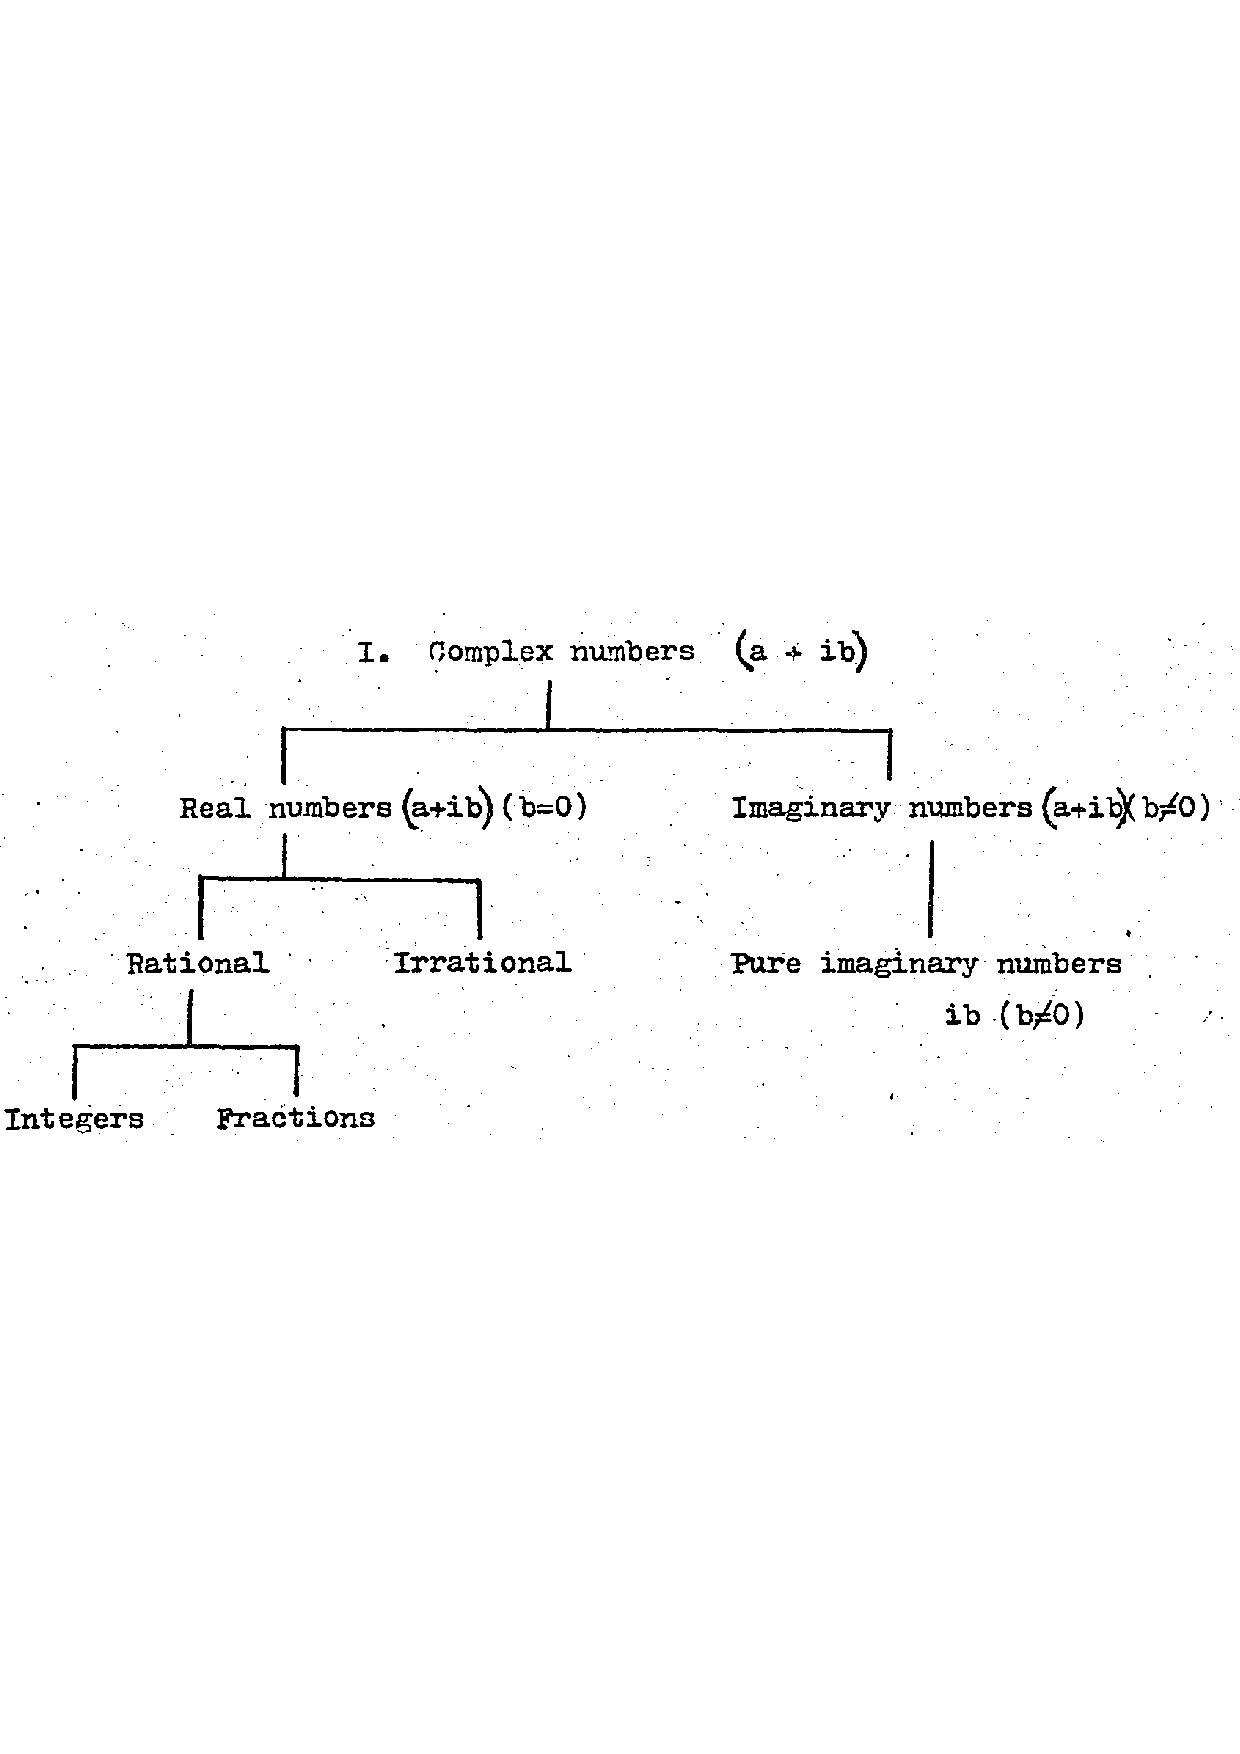
\includegraphics[width=0.9\textwidth]{images/SD-1-1p15A}
%	\caption{Classification of complex numbers}
%	\label{fig:classificationOfComplexNumbersA}
%\end{figure}

%\begin{center}
%\begin{tabular}{cc}
%\end{tabular}
%\end{center}

%\begin{exmp}
%\begin{hSolution}
%\end{hSolution}
%\end{exmp}

%\begin{hEnumerateAlpha}
%\end{hEnumerateAlpha}

%\begin{hEnumerateRoman}
%\end{hEnumerateRoman}

%$
%\begin{bmatrix}
%\end{bmatrix}
%$

%\frac{aaaa}{bbb}
%\frac{a_{n}}{b_{n}}
%\left( aaaa \right)
%\Longrightarrow

%\begin{multicols}{2}
%	bb
%\columnbreak
%	aa
%\end{multicols}
